\documentclass{article} 
\usepackage[left=0.75in,top=0.6in,right=0.75in,bottom=0.6in]{geometry} % Document margins
\usepackage{tabularx}
\usepackage{fancyvrb}
\usepackage{graphicx}
\usepackage{multicol,caption}
\usepackage{fancyhdr}
\usepackage{lipsum}
\usepackage{mathtools}
\usepackage{float}
\usepackage{textcomp}

%Header Stuff
\newenvironment{Figure}
  {\par\medskip\noindent\ignorespaces\minipage{\linewidth}}
  {\endminipage\par\medskip}

\usepackage{fancyhdr}
\pagestyle{fancy}
\fancyhf{}
\renewcommand{\headrulewidth}{0pt}
\fancyhead[R]{\thepage}


\begin{document}

%----------------------------------------------------------------------------------------
%		 TITLE 
%----------------------------------------------------------------------------------------
\begin{center}

\vspace* {15 pt}
\Huge{\bf Performing real time video processing using DE2-115 FPGA}\\
\vspace {20 pt}
\large{Howard Edwards, Michael Micros, Jonathon  Rigney, Megan Rowland \\}

\end{center}

\vspace{15 pt}




\begin{multicols*}{2}

%----------------------------------------------------------------------------------------
%		ABSTRACT
%----------------------------------------------------------------------------------------
{\bf  \textit {Abstract(Jonathon Rigney)} ---}
\par This report is a part of a series of papers aimed at designing and implementing a system to perform real time video processing using a Field Programmable Gate Array(FPGA). This report focuses on the interaction of a user controlled interface(GUI) with the video processing capabilities of an FPGA loaded with the Altera Media Computer and equipped with a camera. The GUI allows the user to adjust the brightness and contrast of the footage being streamed by the camera. This is accomplished on the GUI side by moving a slider. On the FPGA side, the pixels of the frame are taken and their value raised or lowered depending on the operation performed on the GUI’s slider.


{\bf  \textit {Index Terms} --- FPGA, Signal Processing}



%----------------------------------------------------------------------------------------
%		INTRODUCTION
%----------------------------------------------------------------------------------------

\begin{center}
\large{I. Introduction(Howard Edwards)}
\end{center}
\par      The main focus of this report is to document the final stage in the development of a project. The project is the creation of an integrated system that performs the processing of real-time video through a graphical user-interface, GUI, on a computer and the use of field-programmable gate arrays, FPGAs. Detail of the previous stages were documented by Micros, et al [1][2][3][4][5]. During this stage of the project, a camera was added to stream live video, the task of adding an overlay image, and adjusting brightness and contrast is accomplished. 

     The camera used was the Terasic TRDB-D5M camera. The TRDB-D5M is compatible with the DE2-115 board and is connected to the JP5(GPIO) of the board. The system setup remains the same from the previous stage [5] with the camera added. The media computer and the VGA camera controller from a reference design was used to fabricate a FPGA design. This was done through Altera's Qsys design tool. 

     The graphical user-interface and the use of the RS232 communication created from earlier stage[2][5] was used to add an overlay image from the beginning stages[1] [2]  to the video streaming from the camera. The graphical user-interface was also used to adjust the streamed video’s brightness and contrast. The manipulation of the streamed video worked as intended and marked the completion of the overall integrated system.\\

vspace {10 pt}
%----------------------------------------------------------------------------------------
%		DESIGN
%----------------------------------------------------------------------------------------
\begin{center}
\large{II. Design(Megan Rowland)}
\end{center}

{\bf A. Summary of Design--}  
The goal of the design involves modifying the supplied code that enables a camera to output to the VGA port of an Altera Media Computer configured FPGA. The following are the three additions to the supplied code made 1) Add an overlay image to every frame of the video stream 2) Adjust the brightness of the video stream 3) Adjust the contrast of the video stream.


{\bf B. Detail Description}\\
All the image processing performed in the design operates in a very special way due to the circumstances of the design. The processor used was designed by Dr. Lee Belfore (Old Dominion University) using QSys. This processor  is similar to Nios II but additionally incorporates other peripheral components such as the TRDB-D5M CMOS camera. Even though the cideo stream displays perfectly on the monitor using a VGA connection, there was no immediate way to access the data of the video frames being sent to the pixel buffer. Therefore, all image processing was performed by extracting the image already sent to the pixel buffer and performing either the overlay, brightness adjustment or the contras adjustment.\\

\begin{Figure}
 \centering
 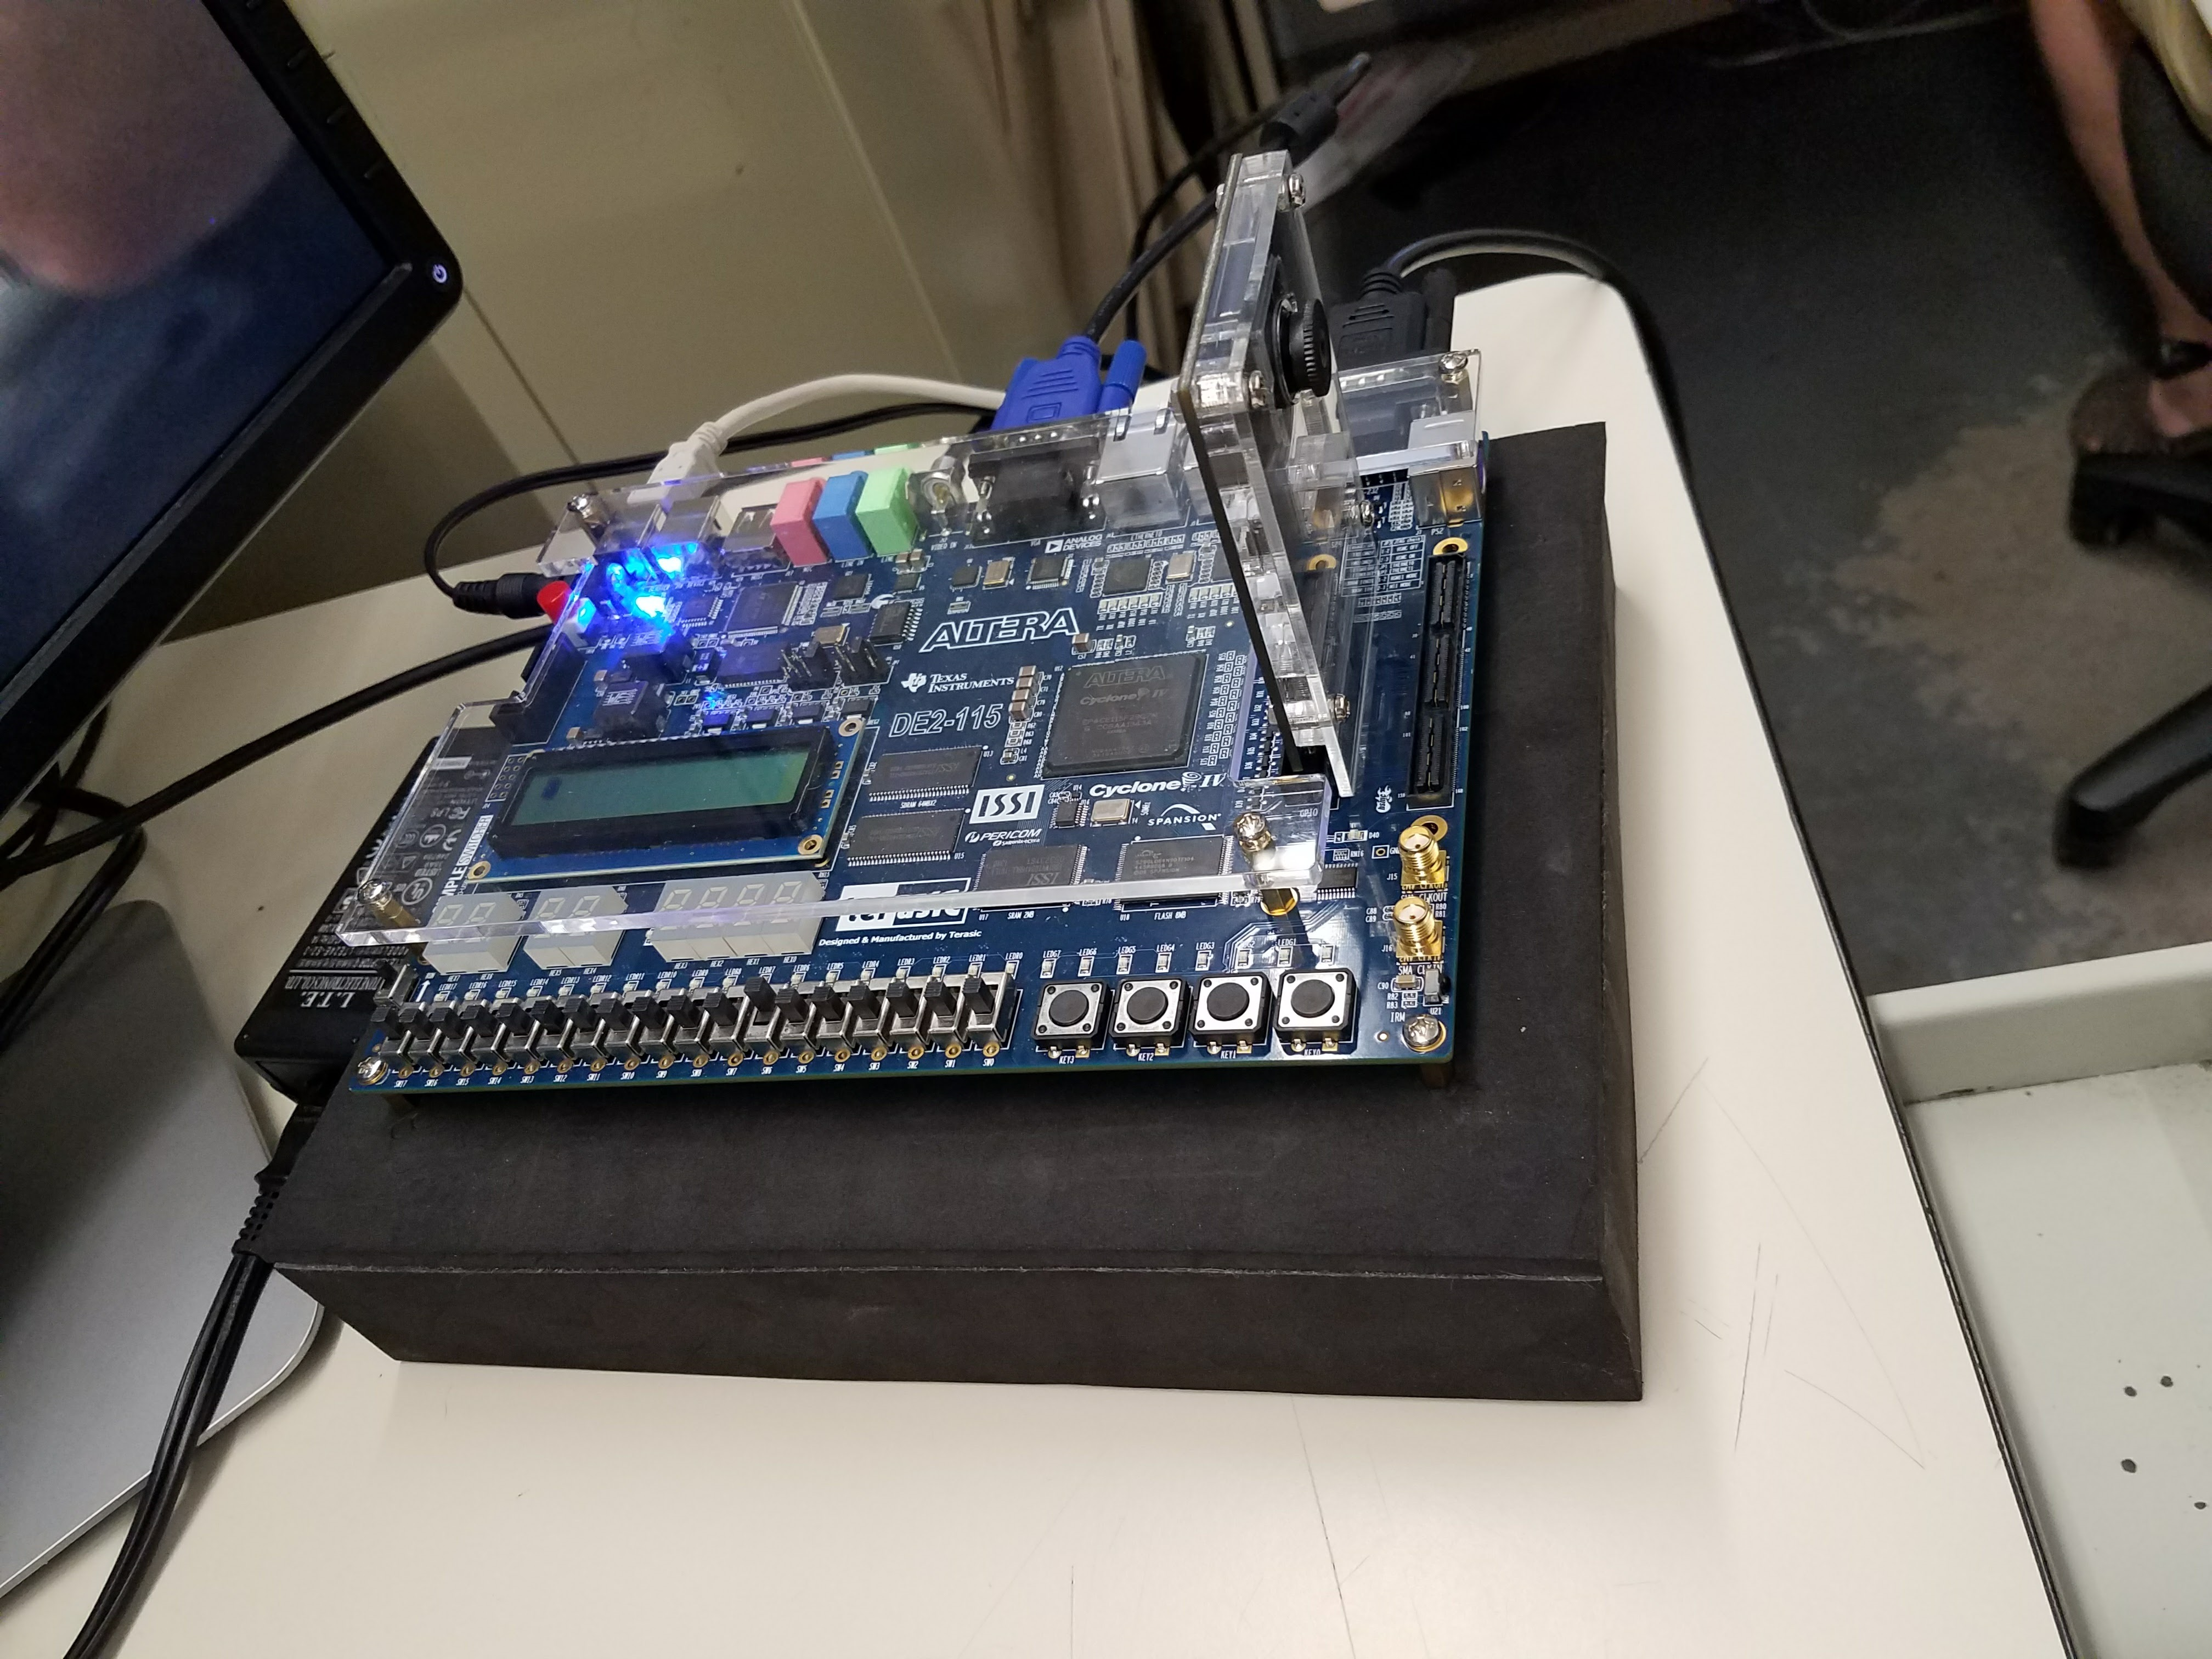
\includegraphics[width=\linewidth]{camera_switch_setup.jpg}
  \captionof{figure} {Layout of the FPGA. Notice the 7th switch from the right is ON.}
\end{Figure}

{\bf  FPGA Set Up: }
 When creating the new project in the Altera Monitor Program, the supplied code was used to configure the System Information File (nios\_system\_sdram\_mod.sopcinfo) and the Quartus II Programming file (DE2\_115\_With\_D5M.sof). These two files configure the FPGA as an Altera Media Computer and extends the architecture to include a camera to pass data through the NIOS processor to the VGA output. When loading the program on the FPGA through Altera Monitor Program, the first 8 switches on the FPGA are used to determine the frame rate of the camera. The following coded functionality is based upon the seventh switch in the on position. This setting allowed a faster frame rate and better picture quality.


The supplied code, capture\_image.c, enables the video output from the camera to display on a monitor wired through the VGA port:

\begin{Figure}
 \centering
 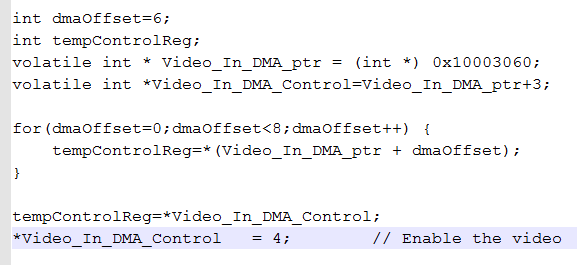
\includegraphics[width=\linewidth]{ccode.png}
\end{Figure}

The overlay image, brightness, and contrast are received through the RS232 port from the QT program as outlined in M. Rowland et al. [5], “Performing image processing on DE2-115 FPGA, controlled by Qt, and displaying to monitor via VGA.”\\

{\bf  Overlay Image: }
Once the overlay image is completely received from the QT program an integer (overlayImageRecieved), is changed from 0 to 1 to indicate the overlay is ready to be written to each frame. The program will then go through a loop every time a new frame is loaded and find the location of  black pixels found in the overlay image and overwrite that same location in the camera frame with white pixels. Each frame from the camera is stored and manipulated in the pixel\_buffer at address 0x08000000:

\begin{Figure}
 \centering
 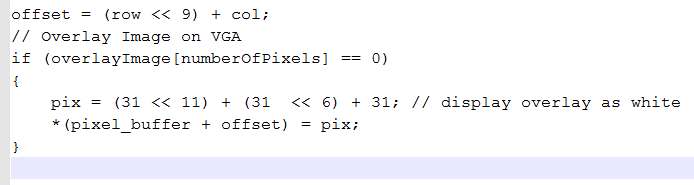
\includegraphics[width=\linewidth]{ccode2.png}
\end{Figure}

{\bf  Brightness: }
Once the brightness slider value is received from the QT program a integer, changeB, is changed from 0 to some value between 1 and 10 or -1 and -10. The changeB integer is calculated based upon the value of the brightness slider value received to increase brightness if the slider is moved to the right or decrease brightness if the slider is moved to the left:

changeB = (brightness - 50)  * 1/5 ;

When changeB is greater than or less than 0, the program will then go through a loop every time a new frame is loaded and increase or decrease the brightness value of each red, green and blue component of each pixel of that frame by changeB and bound the pixel value from 0 to 31 (this is the smallest and largest value a pixel can have).	

\begin{Figure}
 \centering
 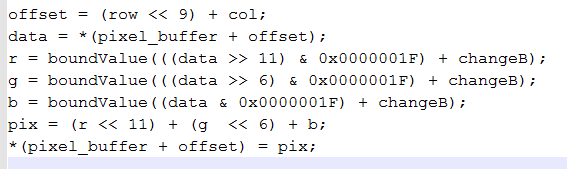
\includegraphics[width=\linewidth]{ccode3.png}
\end{Figure}

{\bf  Contrast: }
Once the contrast slider value is received from the QT program a integer, changeC, is changed from 0 to some value between 1 and 10 or -1 and -10. The changeC integer is calculated based upon the value of the contrast slider value received to increase contrast if the slider is moved to the right or decrease contrast if the slider is moved to the left (calculated the same as changeB).
When changeC is greater than or less than 0, the program will then go through a loop every time a new frame is loaded and increase or decrease the contrast value of each pixel of that frame. In order to increase or decrease contrast a float, factor, is calculated between 0.5 and 1.95 by the following equation:

factor = (34.0 * (changeC + 31.0)) / (34.0 * (31.0 - changeC));

If the factor is less than 1, then the contrast is decreased. If the value is greater than 1, then the contrast is increased. Each red, green and blue component of each pixel value for each frame is then multiplied by the factor value to increase or decrease contrast accordingly:

\begin{Figure}
 \centering
 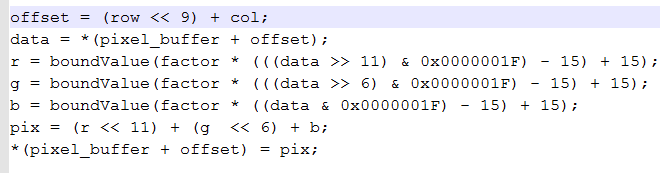
\includegraphics[width=\linewidth]{ccode4.png}
\end{Figure}


%----------------------------------------------------------------------------------------
%		EVALUATION
%----------------------------------------------------------------------------------------
\begin{center}
\large{III. Evaluation(Michael Micros)}
\end{center}

The video processing performed as expected under the special circumstances of the implementation. As mentioned in the Design section, the image processing was performed after a new frame was writen to the pixel buffer and displayed to the monitor. Therefore, it is expected that any action taken would be rather slow or happen very obviously after the image is shown on the monitor. This was not the case for the overlay performed, as it seemed to happen rather instantaneously at slower frame rates.

\begin{Figure}
 \centering
 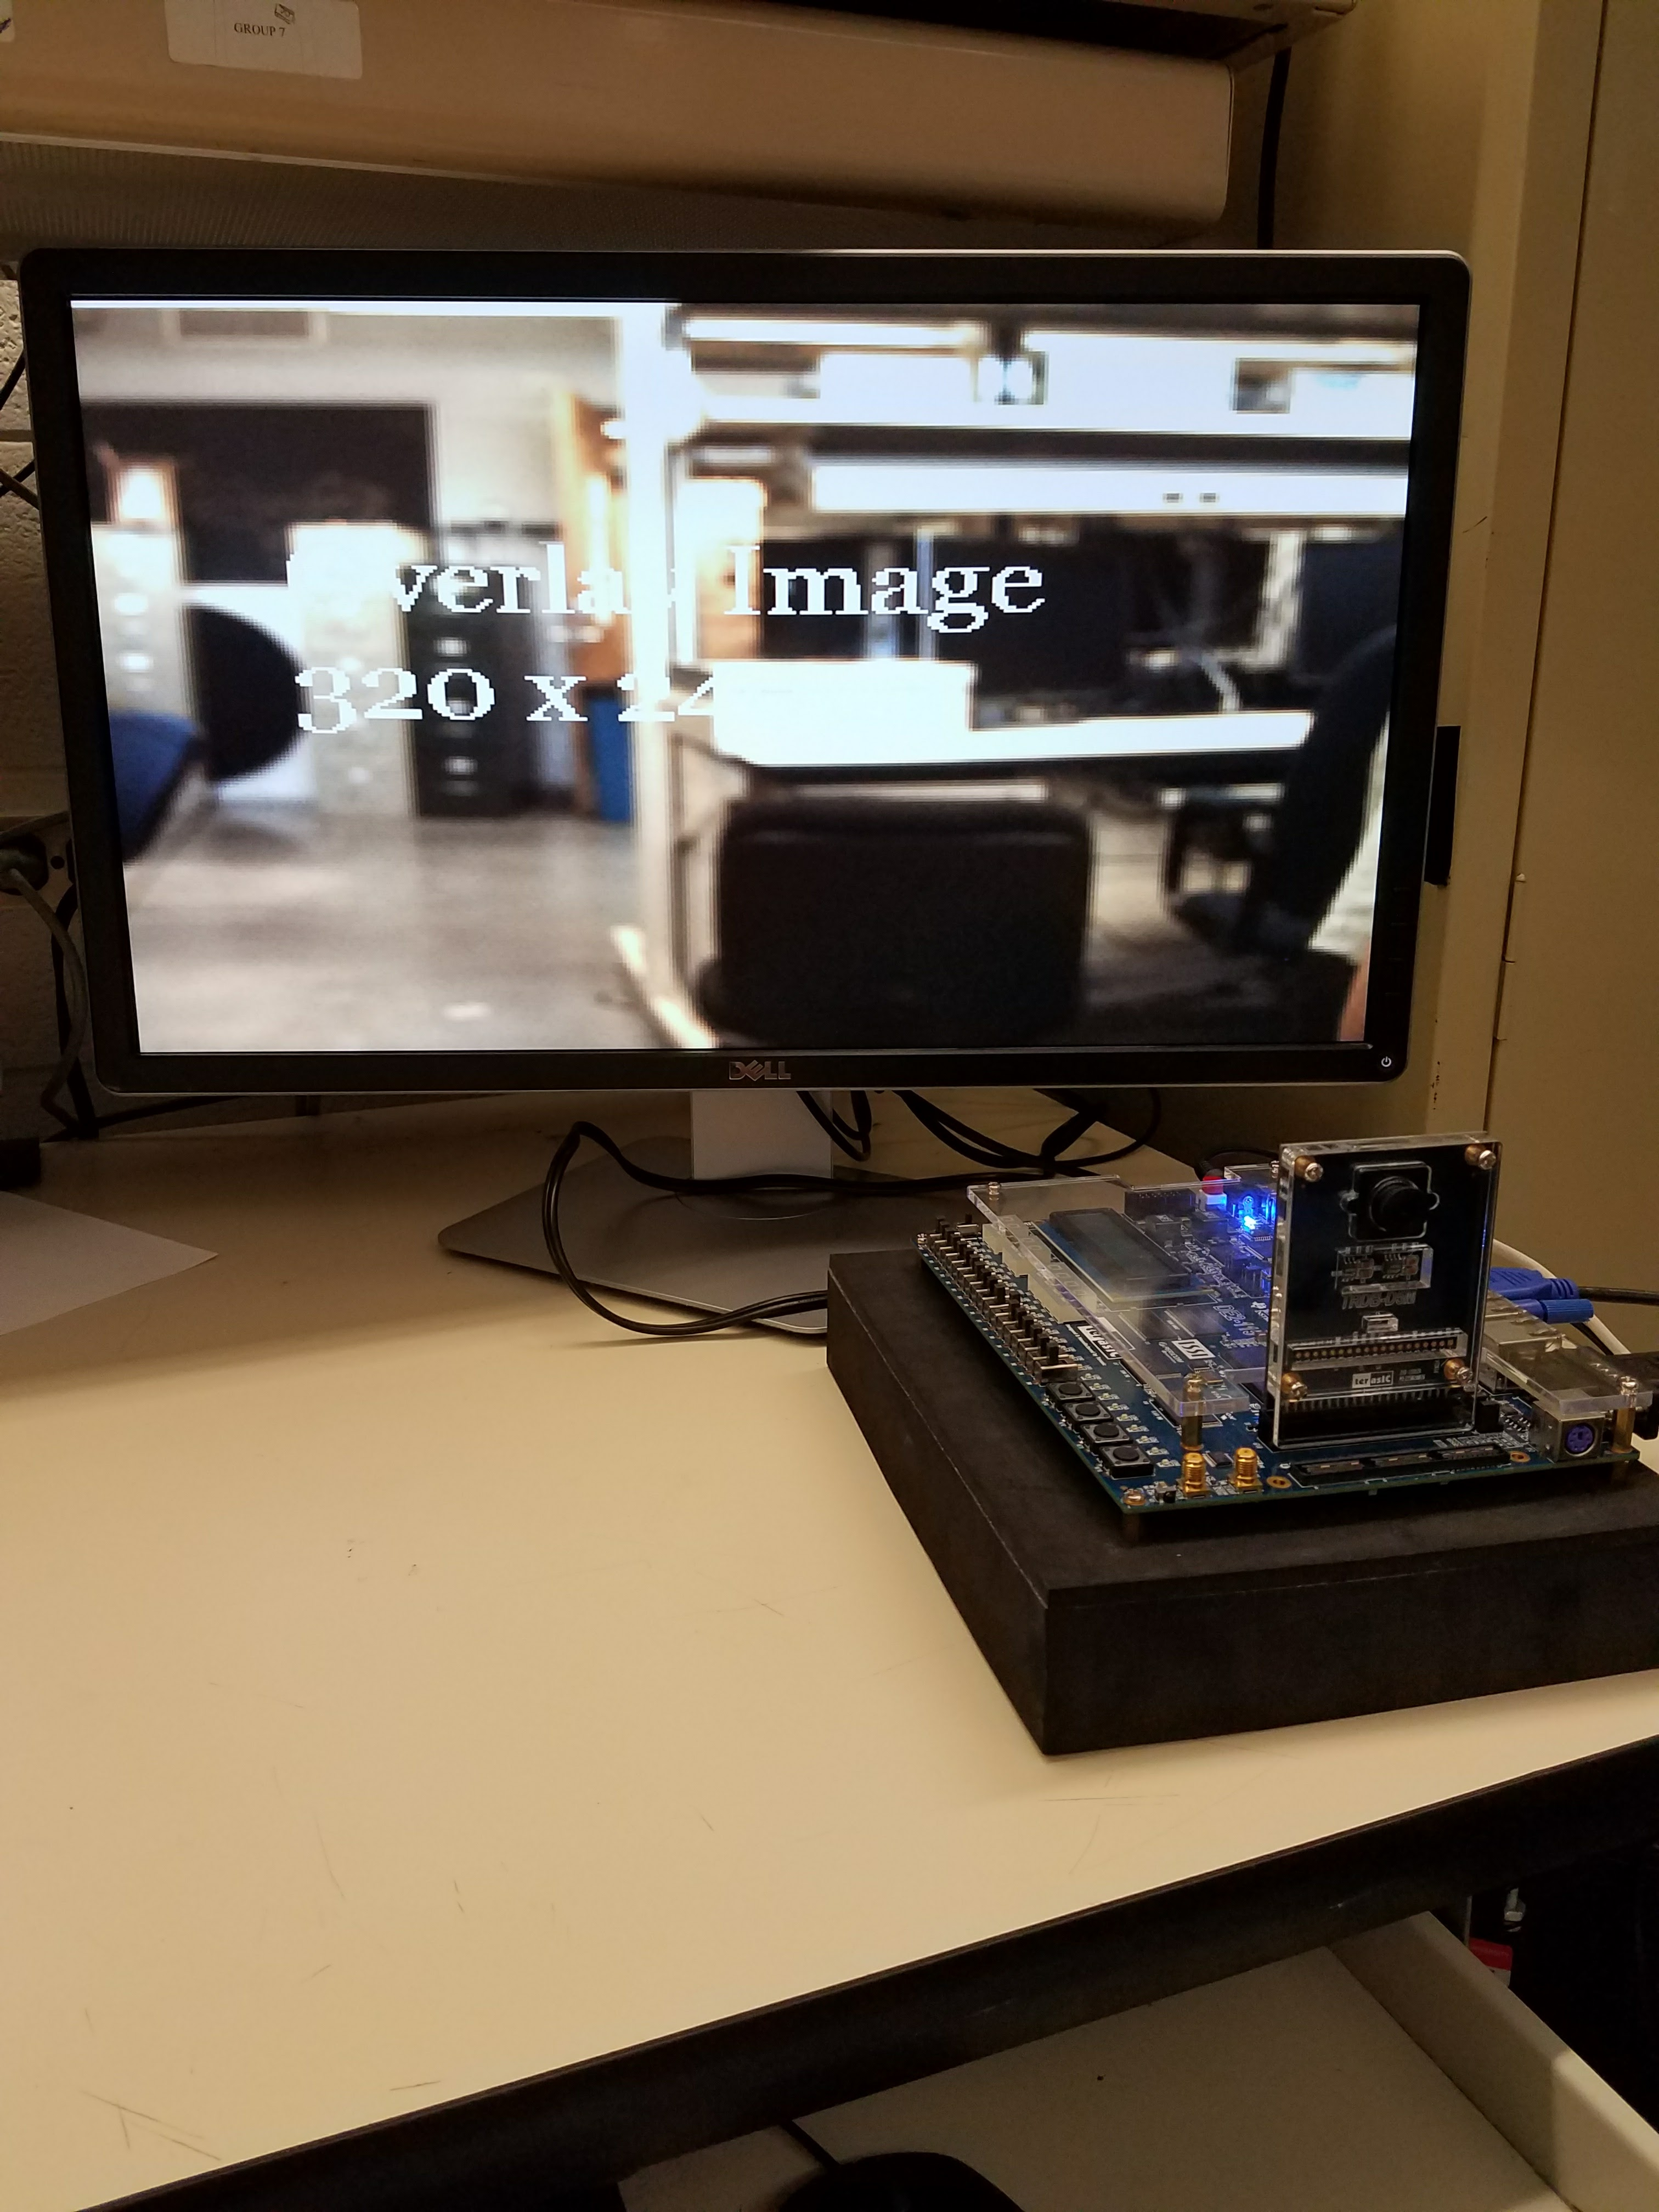
\includegraphics[width=\linewidth]{overlay_image.jpg}
\captionof{figure} {Text overlaid on top of video stream.}
\end{Figure}

The brightness adjustment performed was noticeably slower due to the added complexity in the processing. As a result the brightness adjustment is visible as it is performed starting from the top of the frame and moving down. This can be seen in the following image where the frame is made brighter but has only done so for the top half of the frame, since it is still in the process of adjusting the brightness.

\begin{Figure}
 \centering
 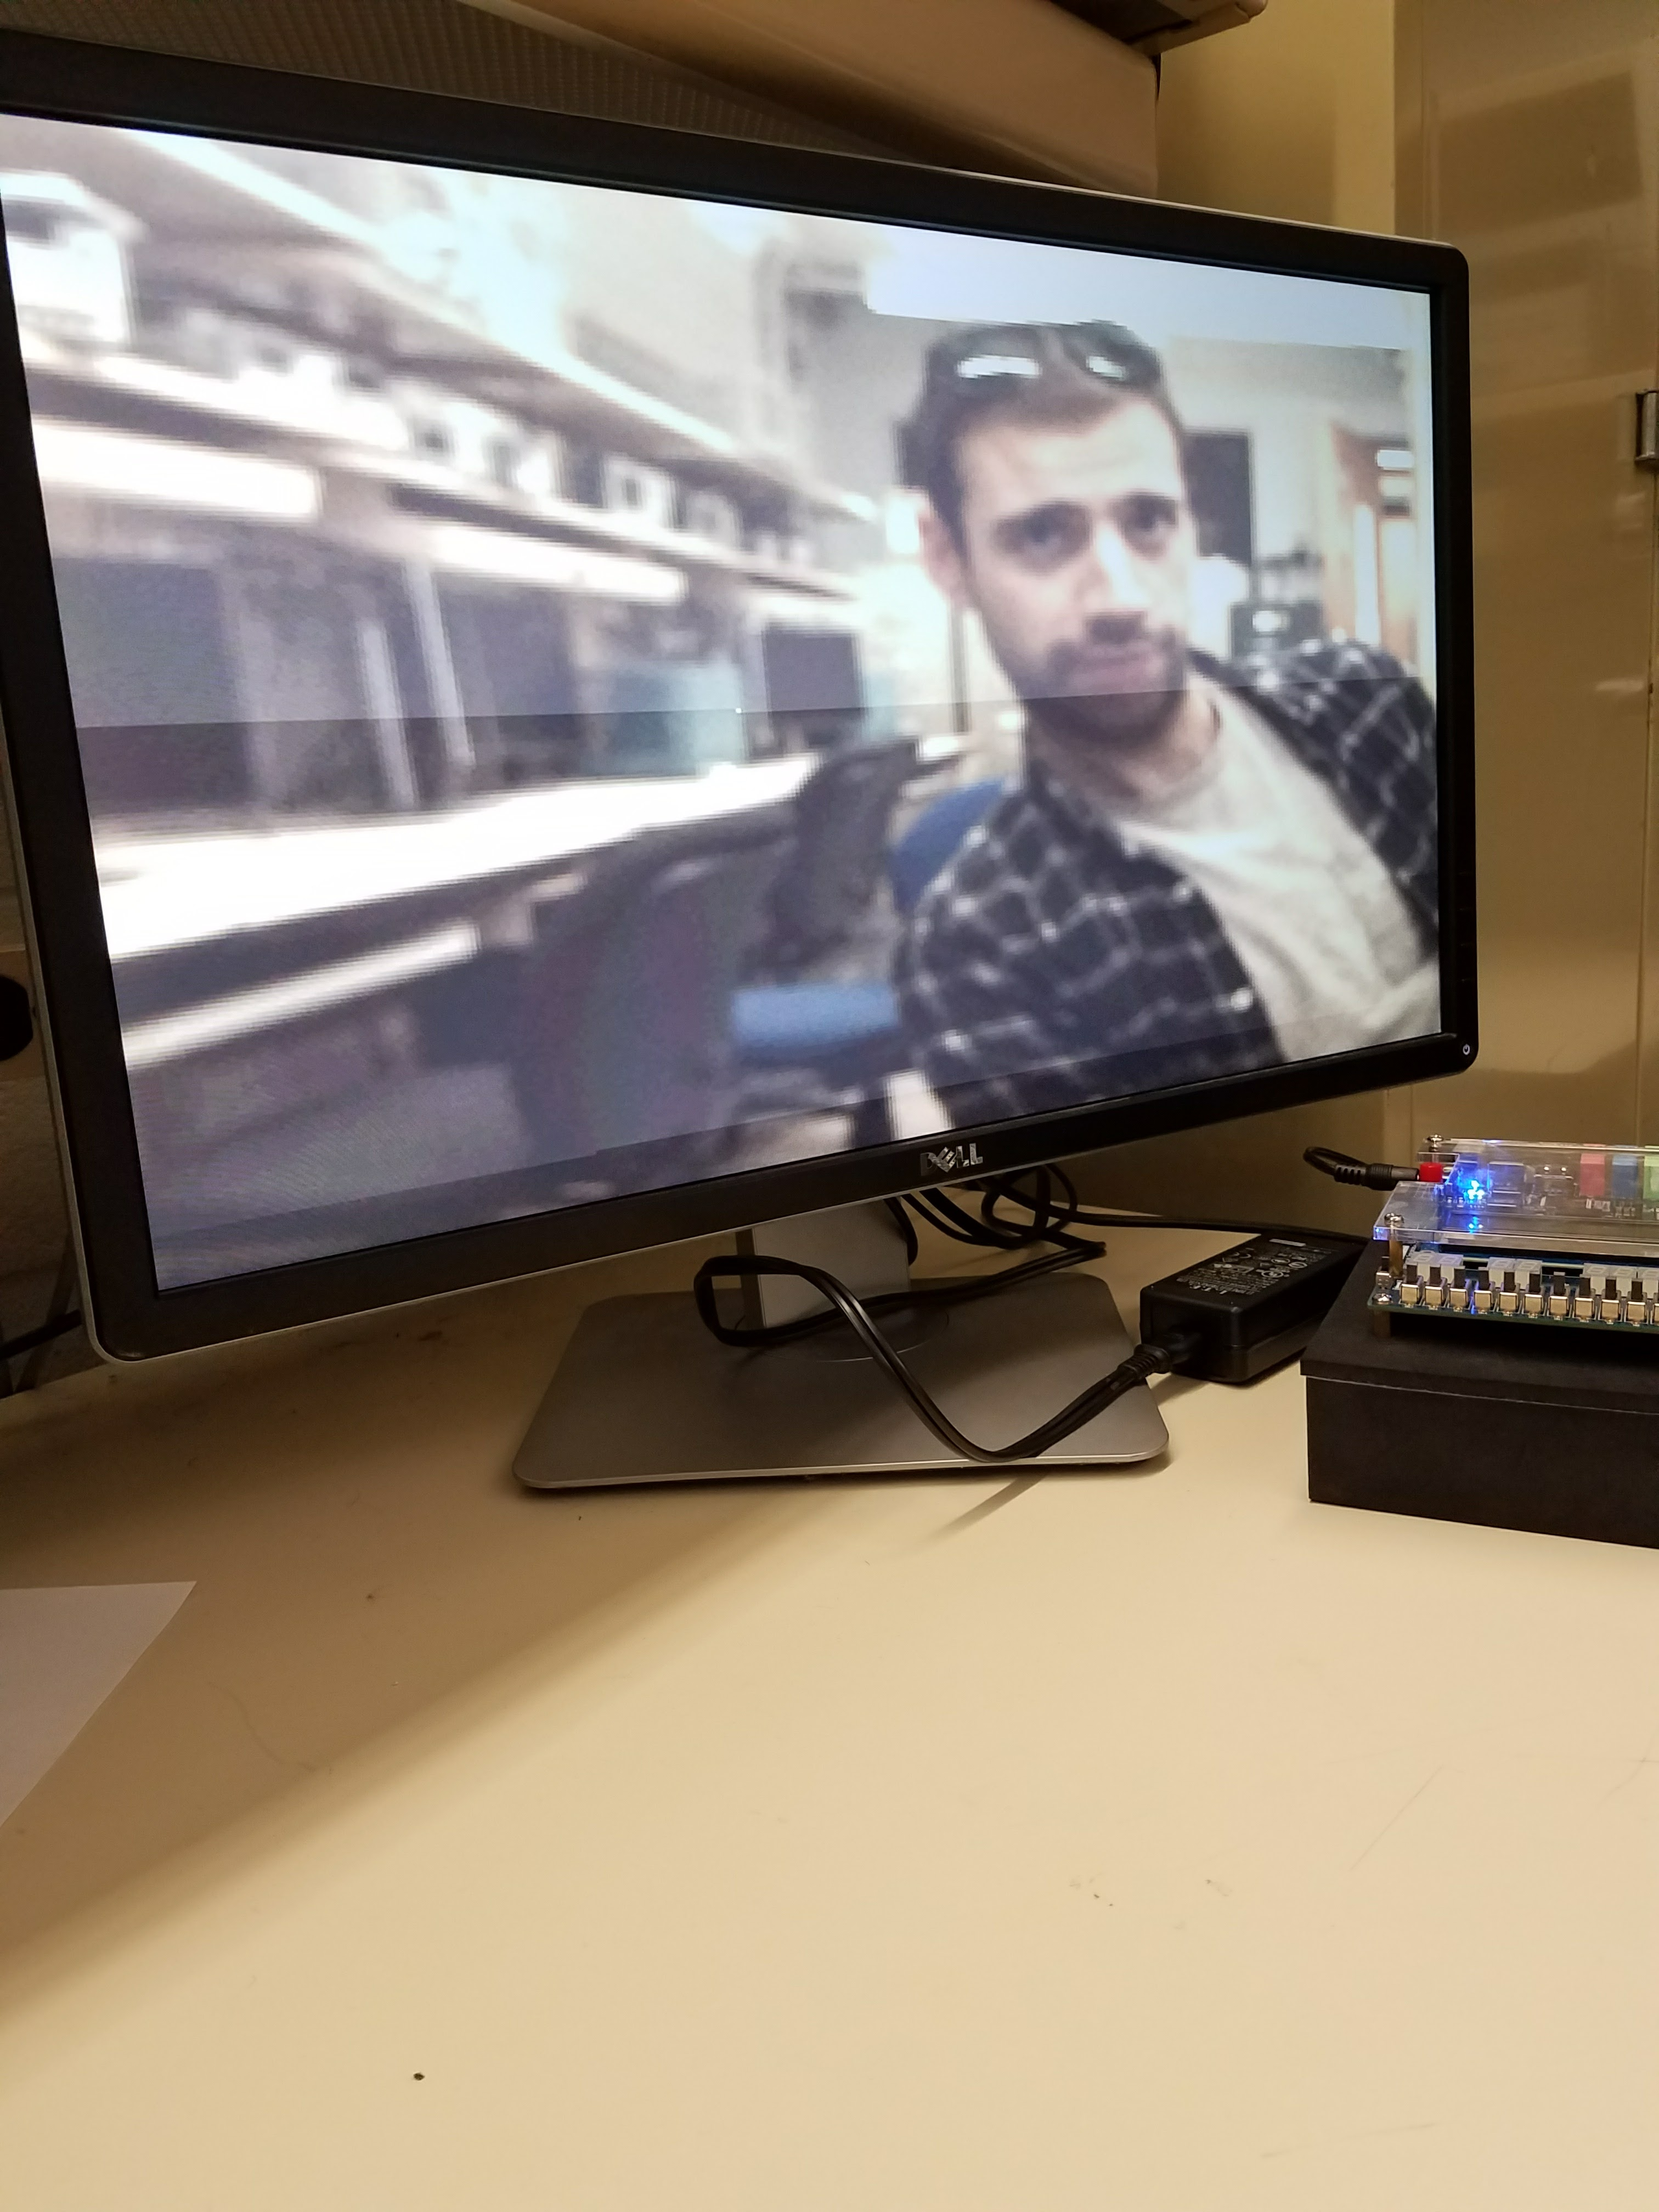
\includegraphics[width=\linewidth, height = 10 cm]{brightness_increase.jpg}
\captionof{figure} {Performing brightness adjustment(Making frame brighter).}
\end{Figure}

\begin{Figure}
 \centering
 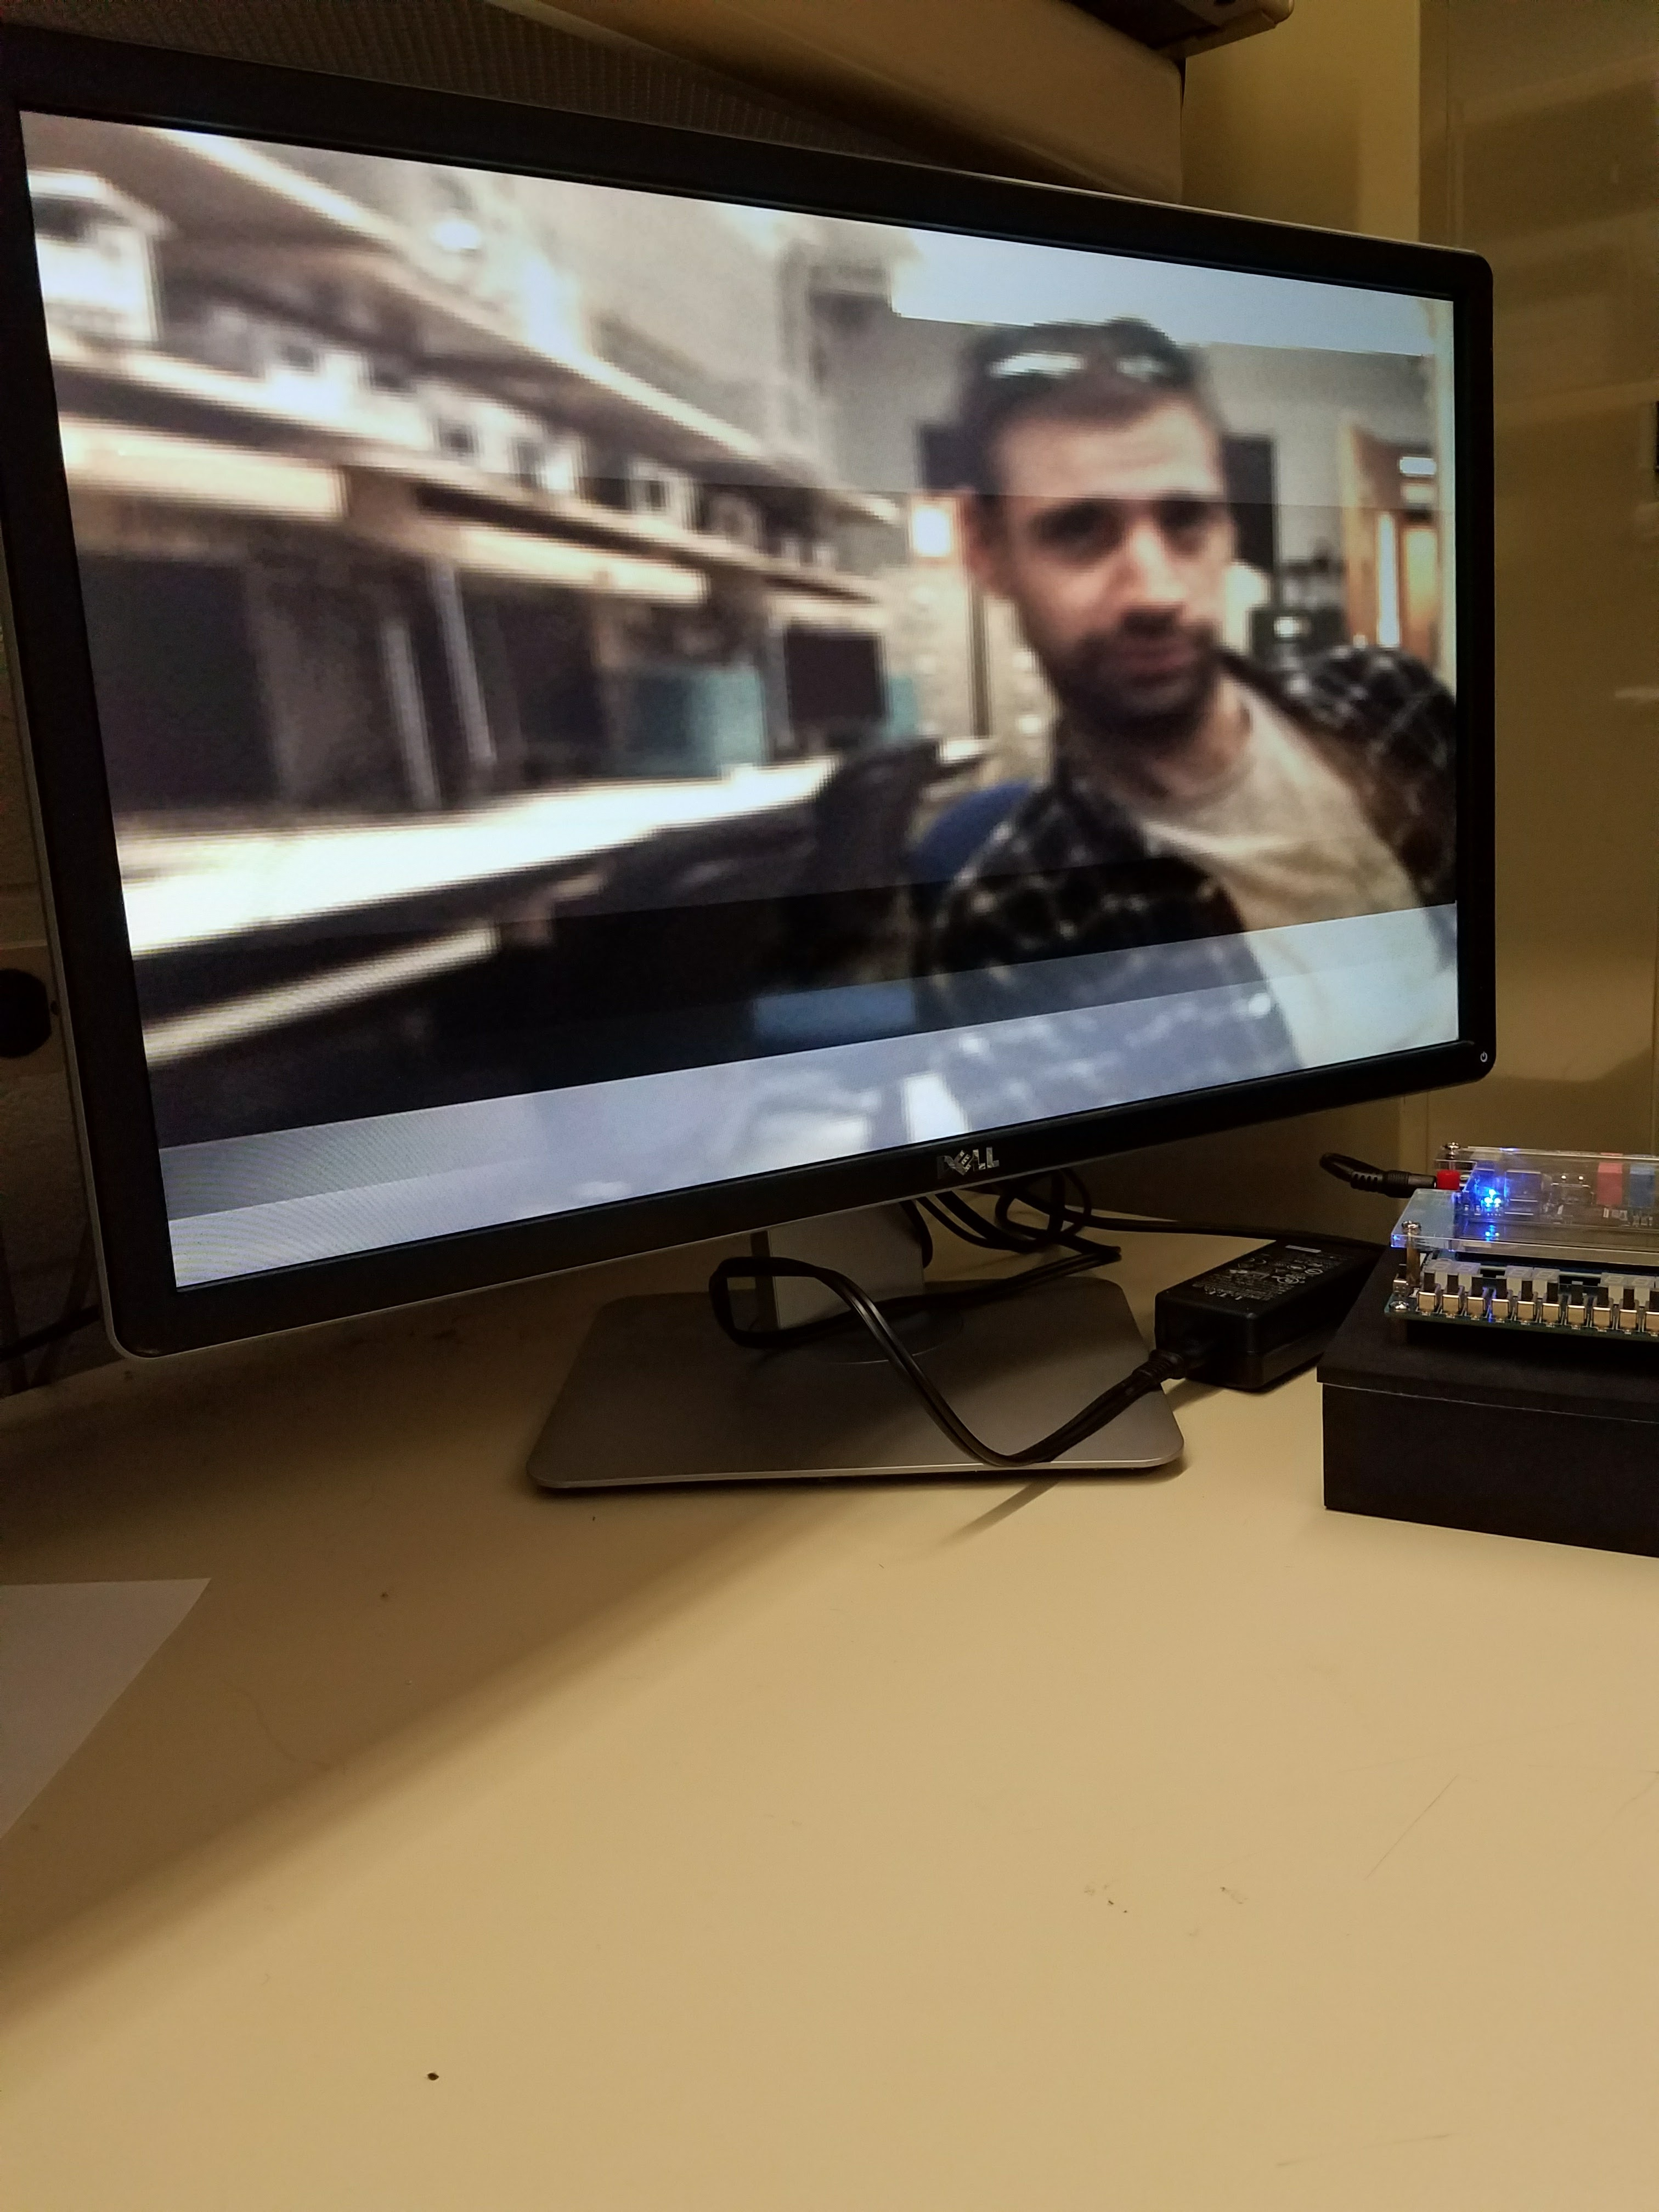
\includegraphics[width=\linewidth, height = 10 cm]{brightness_decrease.jpg}
\captionof{figure} {Performing brightness adjustment(Making frame darker).}
\end{Figure}

When performing contrast adjustment, the lag between a new frame being loaded and video processing became much more apparent, since contrast adjustment is the most processing intensive of the techniques used. The contrast adjustment requires so much time that a new frame is loaded before the whole frame is processed, leading to the result seen in Fig. 5 where only a part of the frame is adjusted. Then a new frame is loaded in, but the contrast adjusment continuous from the pixel it was last performing the processing on.

\begin{Figure}
 \centering
 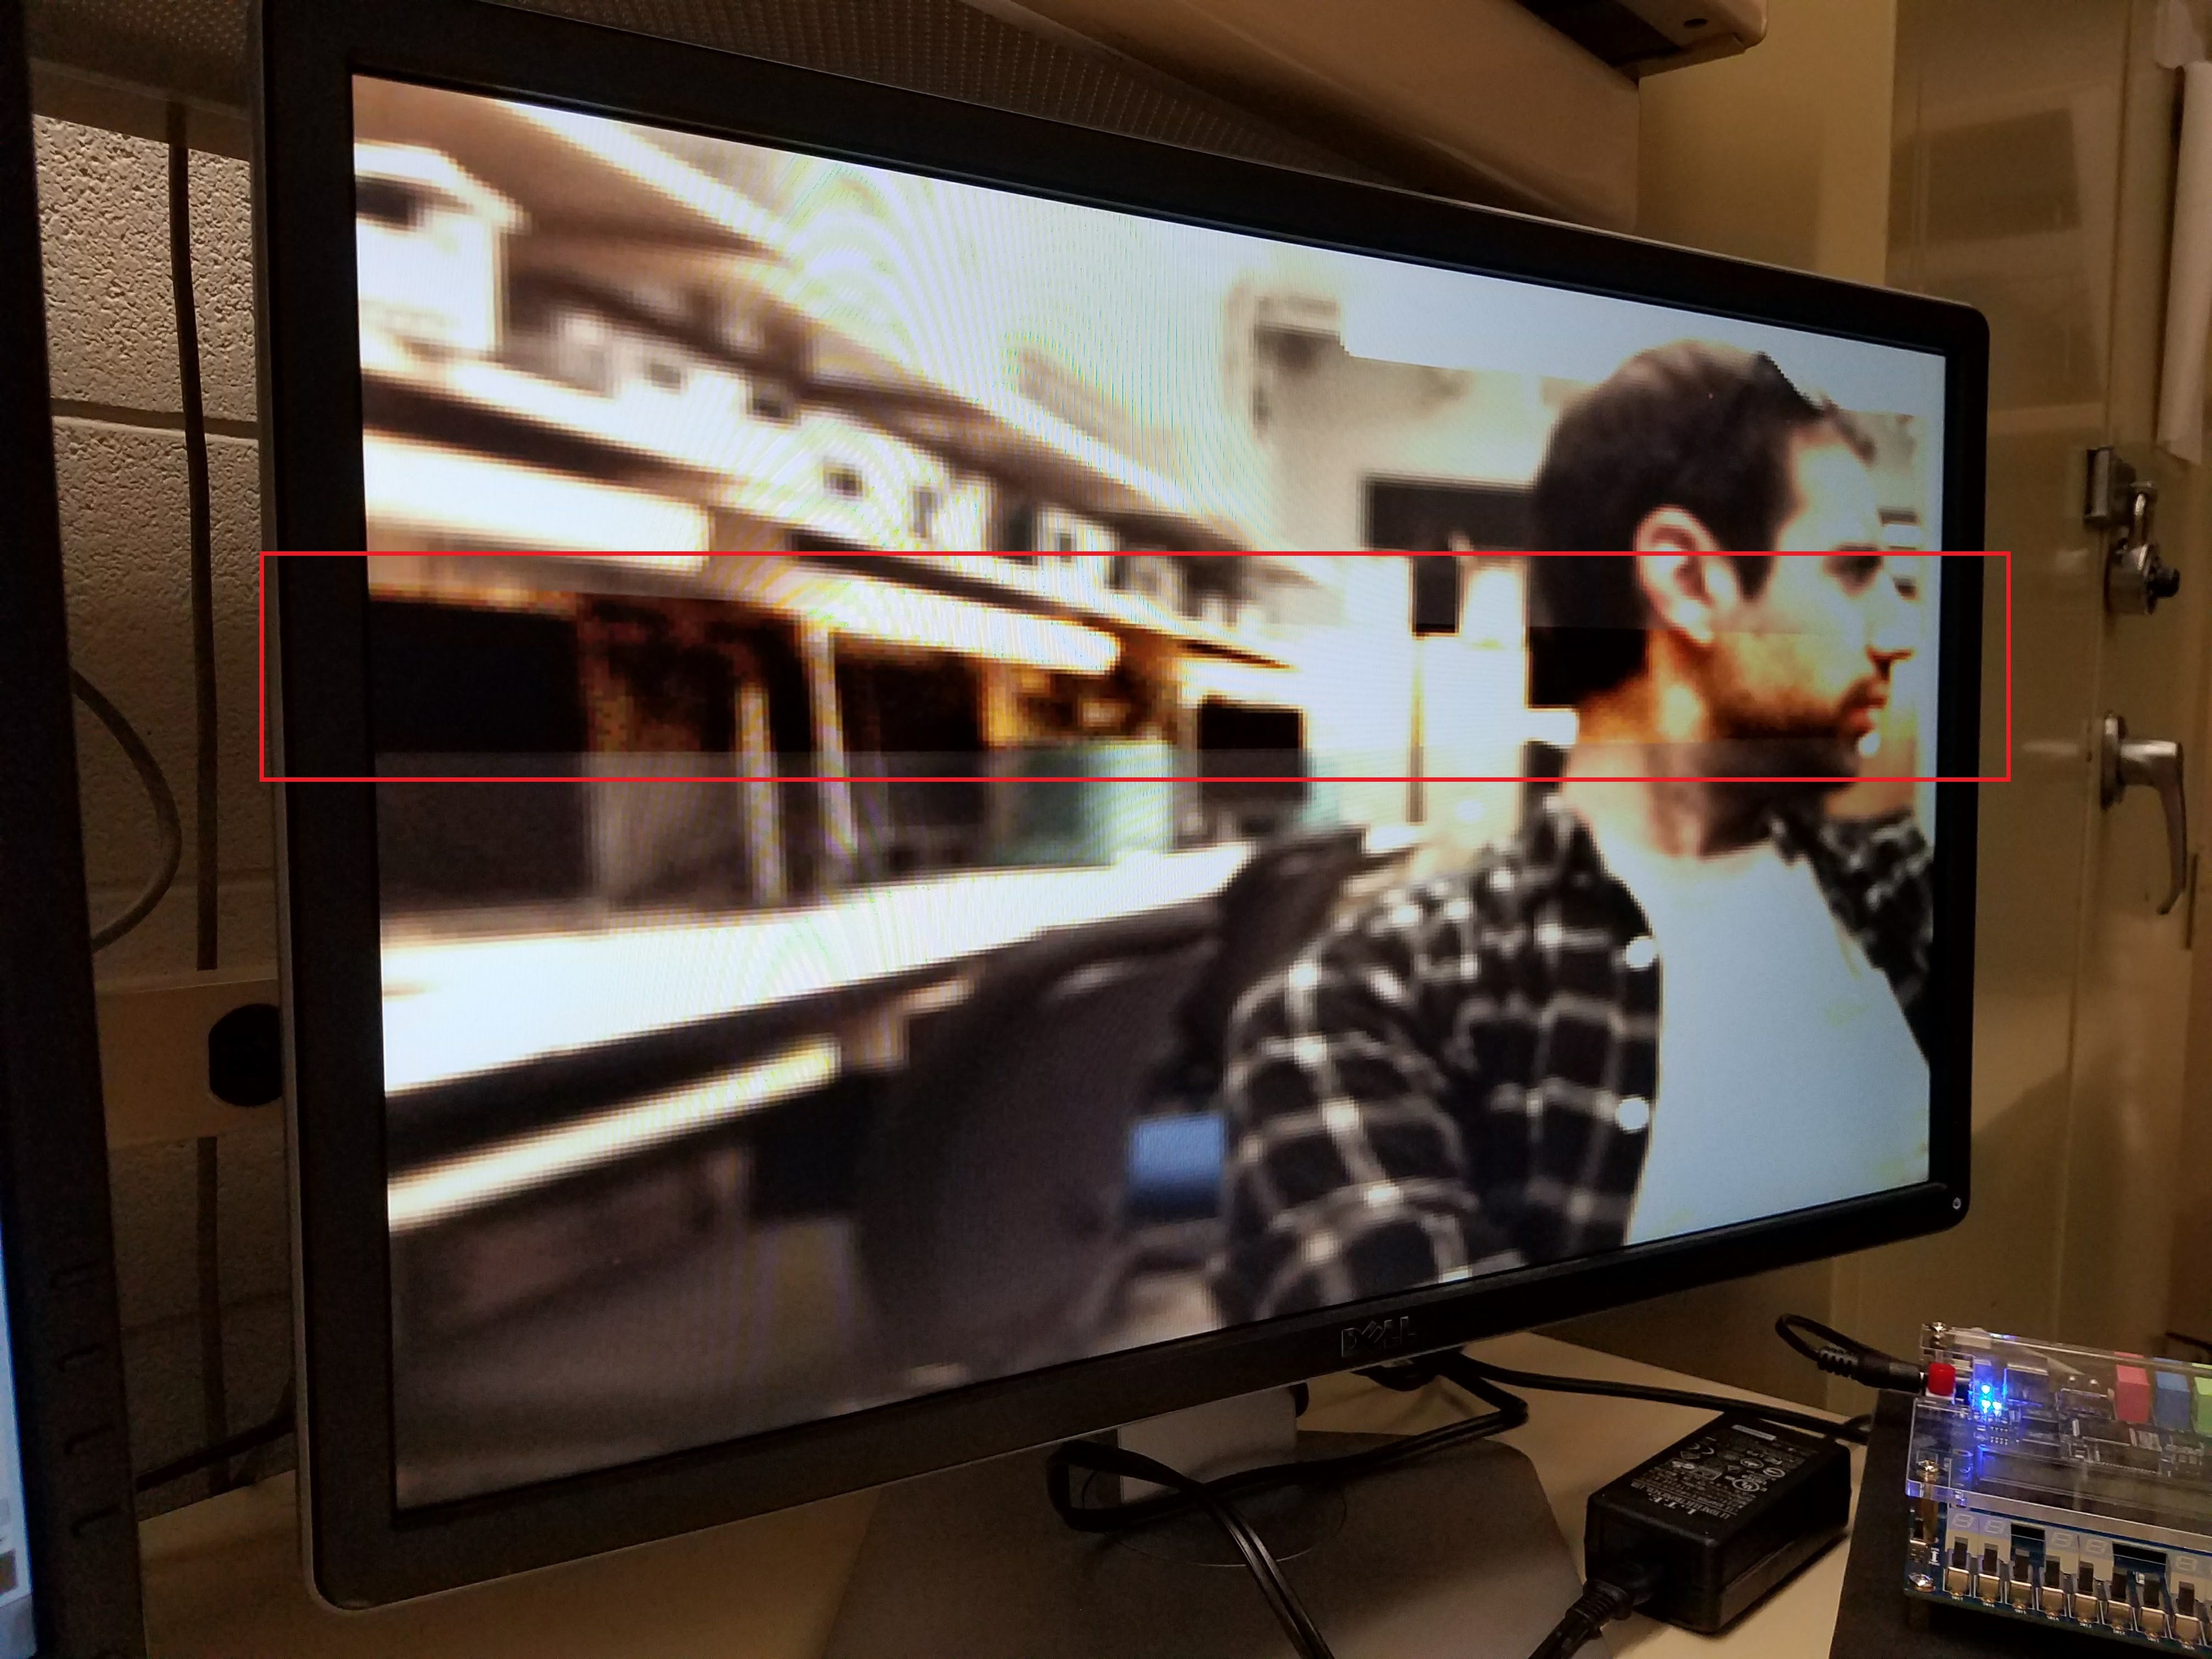
\includegraphics[width=\linewidth, height = 10 cm]{contrast_increase.jpg}
\captionof{figure} {Performing contrast adjustment(higher contrast).}
\end{Figure}

%----------------------------------------------------------------------------------------
%		DISCUSSION
%----------------------------------------------------------------------------------------
\begin{center}
\large{IV. Discussion(Michael Micros)}
\end{center}

Obviously, the performance of our video processing design can be improved, but this requires a great understanding of FPGAs in order to be able to extract the data recorded by the camera. If accessing that data were possible, the data would first be prcessed to perform image overlay, brightness and contrast adjustment, and only after the processing was done would the video frame be displayed on the monitor.

 Some notable problems we had to overcome were related to the task of brightness adjustment. In order to increase or decrease the brightness of an RGB image the same value must be added to all three color bins. A small logical error caused unexpected results and took our team about 2 hours to debug. Once this error was corrected all other aspects of our project functioned as expected.




%----------------------------------------------------------------------------------------
%		REFERENCES
%----------------------------------------------------------------------------------------
\begin{center}
\large{IV. References}
\end{center}

[1]	H. Edwards et al., “Image Processing: Overlaying and Histogram Equalization,” Old Dominion University, Norfolk, Virginia, Feb 2017.

[2]     M. Micros et al., “ Creating Graphical User Interface GUI for processing images,” Old Dominion University, Norfolk, Virginia, Feb 2017.

[3]	J. Rigney et al., “Implementing AND gates, 8-bit binary counters and 2-Digit BCD counters using DE2-115 FPGA,” Old Dominion University, Norfolk, Virginia,  Mar 2017.

[4]	M. Rowland et al.,  Establishing communication between Qt program and DE2-115 FPGA,” Old Dominion University, Norfolk, Virginia, Apr 2017.

[5]  	M. Rowland et al.,“Performing image processing on DE2-115 FPGA”, Old Dominion University, Norfolk, Virginia, Apr 2017.
\end{multicols*}


%----------------------------------------------------------------------------------------
%		APPENDIX
%----------------------------------------------------------------------------------------


%----------------------------------------------------------------------------------------
\end{document}
